\documentclass[10pt]{beamer}
\usepackage{xmpincl}
\includexmp{license}
\usepackage[T1]{fontenc}
\usepackage[latin1]{inputenc}
\usepackage{ae}
\usepackage[french]{babel}
\usepackage{array, longtable}
\usetheme{Antibes}
\setbeamertemplate{navigation symbols}{}

% for printing
% \usepackage{pgfpages}
% \pgfpagesuselayout{2 on 1}[a4paper,border shrink=5mm]
% \pgfpagesuselayout{resize to}[a4paper,border shrink=5mm,landscape]

\title{CSIC - Software Engineering}

\subtitle{Project Guidelines}
\usepackage{verbatim}

\author{Irfan Hamid - Pablo Oliveira}
\institute{ENST}

\date{19/01/2009}

\begin{document}
\begin{frame}
  \titlepage
\end{frame}

\begin{frame}
  \frametitle{Outline}
  \tableofcontents
\end{frame}

\section{Team Composition}
\begin{frame}
  \frametitle{Team Composition}
  \begin{itemize}
  \item Two teams of 3 persons, one team of 4 persons.
  \item Each team will have:
    \begin{itemize}
    \item 1 leader
    \item 2 or 3 technical member
    \end{itemize}
  \item Leader's responsabilities :
    \begin{itemize}
      \item Responsible for the organisation and communication within the team.
      \item Establishes a project timeline with the help of the team, and assigns
        tasks to each team member.
      \item Ensures that the project advancement is right on schedule.
      \item Conception and implementation work.
    \end{itemize}
  \item Technical member's responsabilities :
    \begin{itemize}
    \item Helps the leader establishing schedule and work assignment.
    \item Gives feedback to the leader and the rest of the team.
    \item Conception and implementation work.
    \end{itemize}
  \end{itemize}
\end{frame}

\begin{frame}
  \frametitle{Technical member's specific roles}
  \begin{itemize}
  \item The version manager:
    \begin{itemize}
    \item Responsible of archiving the documents and the different code versions.
    \item Responsible of setting up a VCS (version control system) that the team
      can use (svn, git, ...)
    \end{itemize}
  \item The quality manager:
    \begin{itemize}
    \item Ensures that all the team members write tests for their modules.
    \item Ensures that all the tests pass, and checks for regressions.
    \item Checks for problems during the integration of different modules.
    \item He may set up a automatic testing framework to ease the task (Junit).
    \end{itemize}

  \item (Only in a four member team) The documentalist:
    \begin{itemize}
    \item Coordinates documentation writing among the team.
    \end{itemize}
  \end{itemize}
\end{frame}

\section{Phases of the project}
\begin{frame}
  \frametitle{Phases of the project}
  Because projects are simple, a waterfall model should work well.

  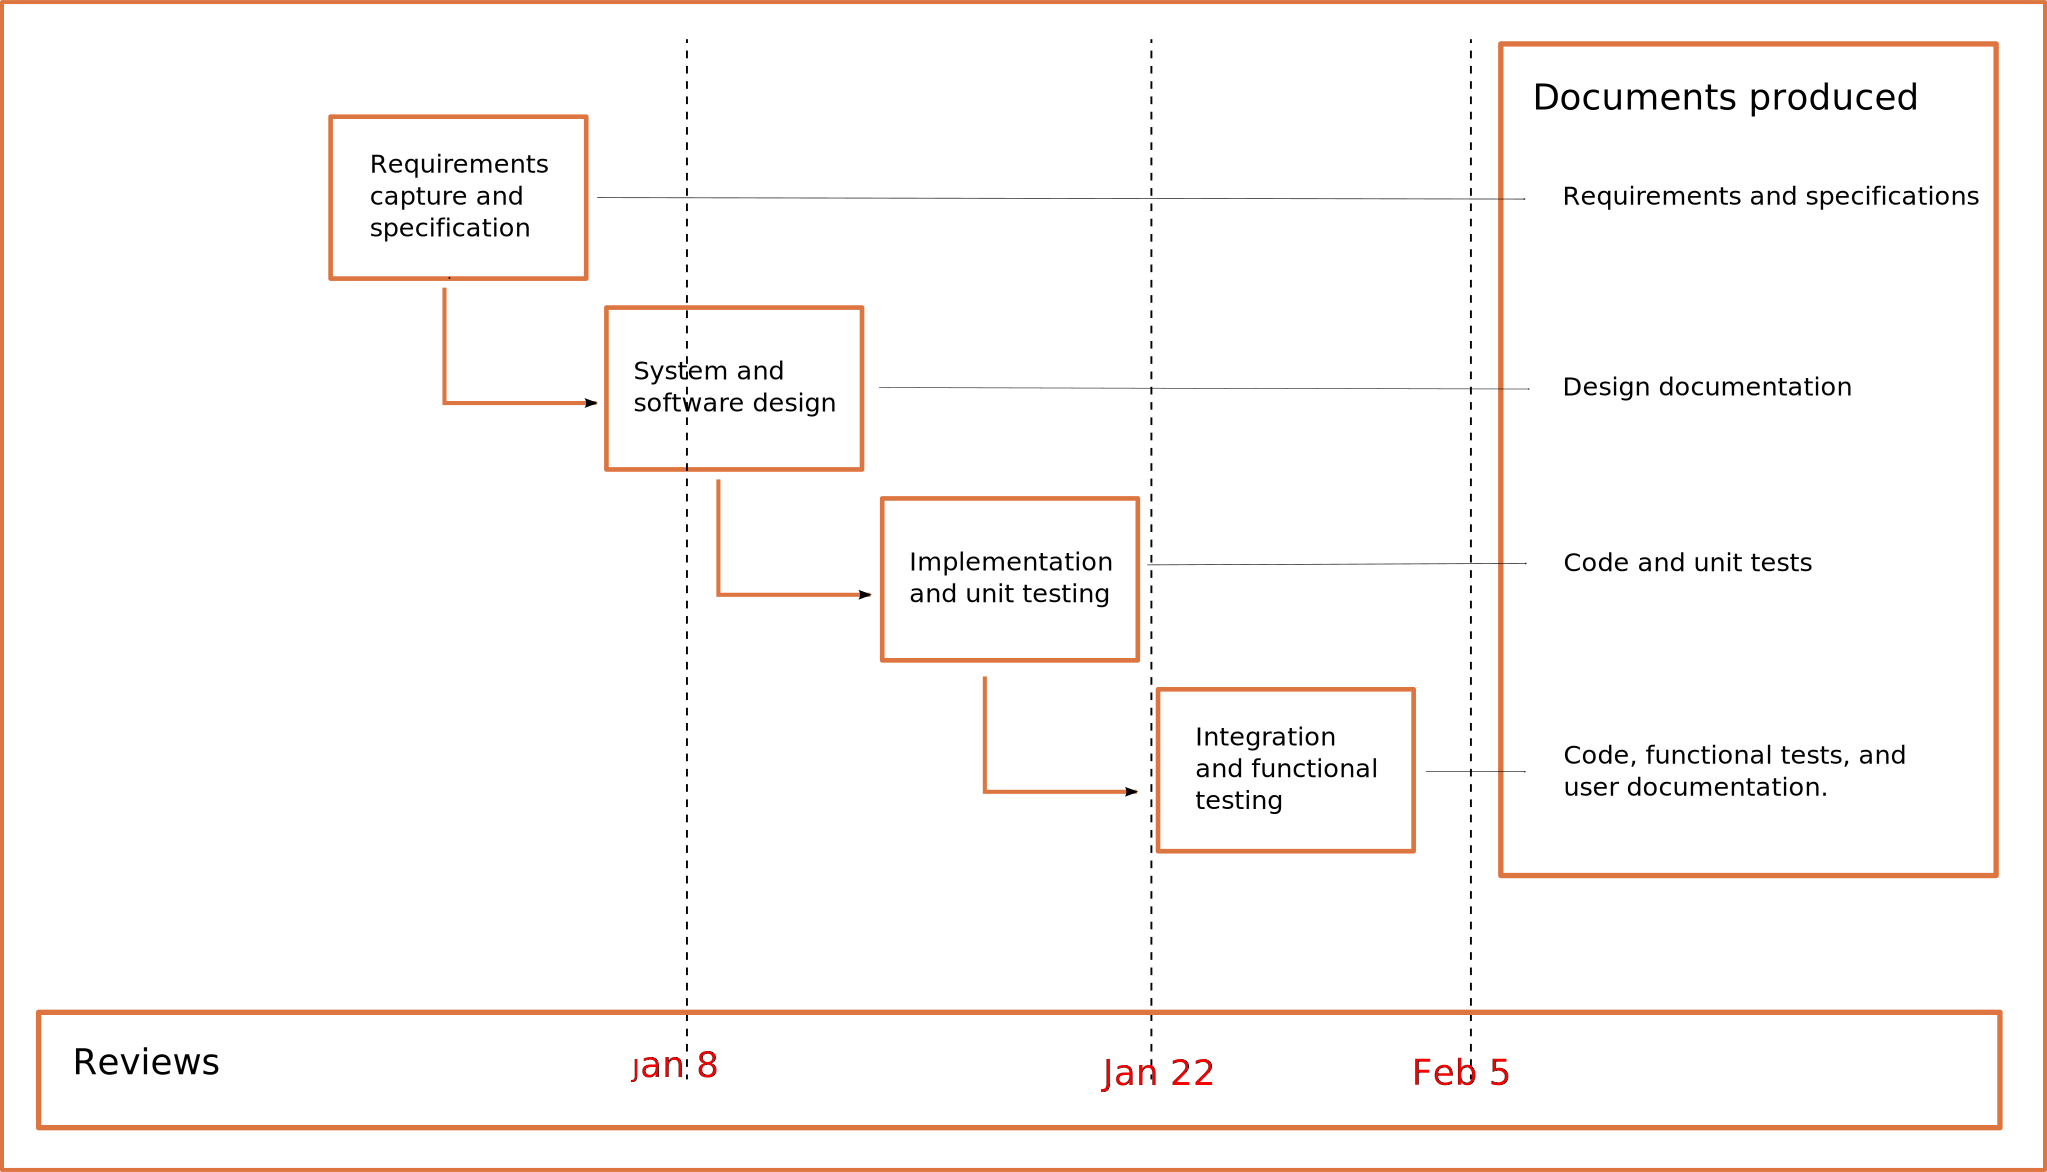
\includegraphics[width=\linewidth]{phases}
\end{frame}

\begin{frame}
  \frametitle{Iterations}
  \begin{itemize}
    \item If you discover a problem in an upstream design phase:
      \begin{itemize}
      \item Document the problem.
      \item Produce an ``Engineering Change Notice'' to correct 
        the upstream specification.
      \end{itemize}
  \end{itemize}
\end{frame}

\subsection{Requirements and specifications}
\begin{frame}
  \frametitle{Requirements and specifications}
  \begin{itemize}
  \item Produce a single document that states requirements and specifications.
  \item There is no imposed format for requirements and specifications (use what
    fits best).
  \item Requirements and Specifications must be numbered and cross-referenced.
    Dependances must be clearly stated.
  \item UML use-case diagrams are welcome to exemplify use-case scenarii.
  \item Do \emph{not} start implementation before finishing specifications.
  \end{itemize}
\end{frame}

\subsection{Design}
\begin{frame}
  \frametitle{Design}
  \begin{itemize}
  \item Think about the different modules that you will need in your project.
  \item Think about the algorithms you will need.
  \item Use UML when appropriate:
    \begin{itemize}
      \item Produce a class diagram for the project.
      \item If needed sequence diagram's can be used.
    \end{itemize}
  \item Once you have identified a decomposition of you application in modules:
    \begin{itemize}
    \item Define their interfaces
    \item Delineate their responsibility.
    \end{itemize}
  \item Write a design document that shows the module decomposition, the
    interfaces and the choice of algorithms. Join a class diagram of your application.
  \end{itemize}
\end{frame}

\subsection{Implementation and unit testing}
\begin{frame}
  \frametitle{Implementation and unit testing}
  \begin{itemize}
  \item Define a coding convention and stick to it.
  \item Code cleanly, factorize (do not duplicate code).
  \item Add \emph{useful} comments to:
    \begin{itemize}
    \item Each class
    \item Each method
    \item Each difficult to understand block of code
    \end{itemize}
  \item Write unit tests while (or before) writing the code.
  \item Use a VCS !
  \item Communicate a lot in the team.
  \end{itemize}
\end{frame}

\subsection{Integration and functional testing}
\begin{frame}
  \frametitle{Integration and functional testing}
  \begin{itemize}
  \item If your interfaces where well defined, integration should be smooth.
  \item Write functional tests for your entire application.
  \item Try corner cases.
  \item Do GUI tests by hand.
  \item Ideally, the person testing a functionality must not be the person who
    wrote it.
  \end{itemize}
\end{frame}

\section{Delivery}
\begin{frame}
\frametitle{Delivery}
\begin{itemize}
\item Expected on time.
\item Should include:
\begin{itemize}
  \item Commented Code
  \item Tests
  \item User Manual
  \item README, that explains how to install and run the application (if needed
    state any external library requirements).
\end{itemize}
\item Good Luck!
\end{itemize}
\end{frame}
\end{document}
